\section{The perf application}
The perf\index{perf} application is part of the Linux kernel tools. The source code is found in the kernel sources in the directory \file{\textless linux source\textgreater /tools/perf/}. perf is comprised of several sub-tools for different tasks. These are for example the recording or reporting of events. Each of these sub-tools acts like an stand alone application, but uses a common infrastructure. The tools are executed with a command line argument for perf, e.g. \console{perf recording -h} or \console{perf report -h}.

\subsection{perf record}
The perf record tool is used to capture events and write them into a data file. By default, the data file has the name \file{perf.data} and is in the current working directory. It was used to capture all applications on all CPU's with timestamps. The command line to achieve this is \console{perf record -a -T}\footnote{But it seems that the \code{-T} flag has no influence on the recording}. To capture on all CPU's, the pseudo file \file{/proc/sys/kernel/perf\_event\_paranoid} has to have the content \code{0} or \code{-1}.

During recording, several occurrences of an event are reported together. There exist two different modes. In the default case, the Kernel tries to measure 1000 samples per second. Therefore, it adjusts the sampling period dynamically \cite{kernel.org2011}. With the switch \code{-c <n>}, a sample is generated for $n$ events.

Figure \ref{fig:perfRecord} gives an overview how the recording works. First perf record initializes the recording via the perf\_events interface of Linux. The records are then written into mmap pages\footnote{not to confuse with the mmap record, they both have the same name} and a signal is sent to perf record if a page is full. perf record then stores the records into the data file.

\begin{figure}[ht]
  \center
  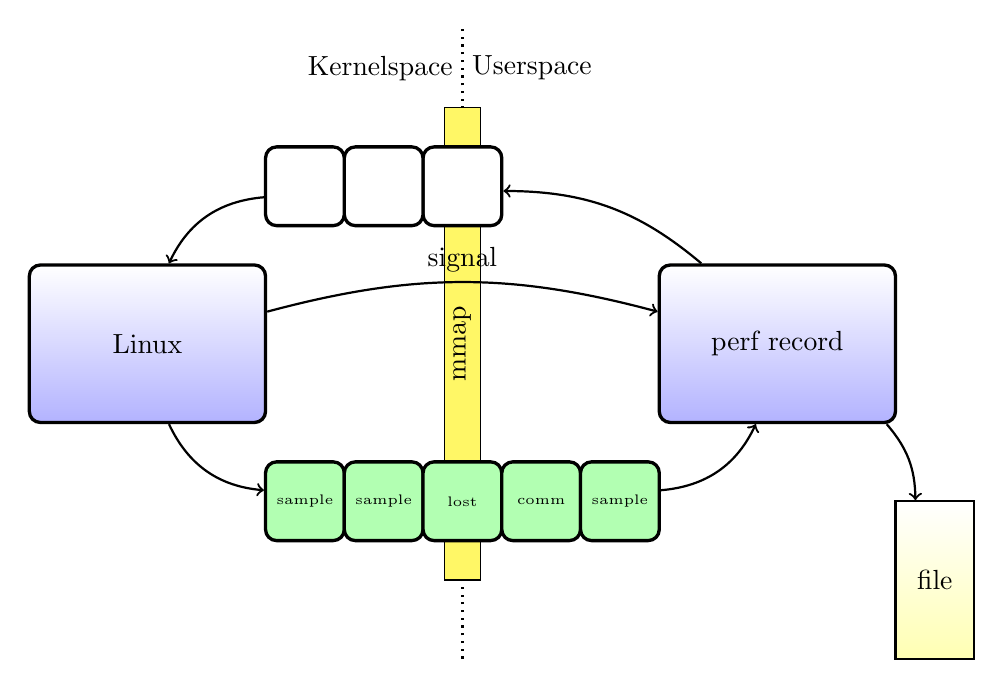
\begin{tikzpicture}[scale=1,transform shape]
\tikzstyle{app}=[anchor=center,minimum width=3 cm,minimum height=2 cm,rectangle,rounded corners,draw=black, top color=white, bottom color=blue!30,very thick, text centered]
\tikzstyle{map}=[anchor=center,minimum width=1 cm,minimum height=1 cm,rectangle,rounded corners,very thick, text centered,draw=black,fill=white]
\tikzstyle{event}=[map, fill=green!30,very thick, text centered]
\tikzstyle{arrow}=[->,thick]
\tikzstyle{Interface}=[rectangle,draw=black, fill=yellow!60,rotate=90]
\tikzstyle{file}=[anchor=center,draw=black, top color=white, bottom color=yellow!30,thick, text centered]


\path [thick, dotted] (0,-4) edge (0,4);
\node [anchor=east] at (0,3.5) ()  {Kernelspace};
\node [anchor=west] at (0,3.5) ()  {Userspace};
\node [Interface,minimum width=6 cm] at (0,0) (iface) {mmap};

\node [app] at (-4,0) (linux)  {Linux};
\node [app,minimum width=3 cm,minimum height=2 cm] at (4,0) (perf)  {perf record};

\path [arrow,bend right=-15] (linux) edge node[above]{signal} (perf);

\node  [event] at (-2,-2) (ev0) {\tiny{sample}};
\node  [event] at (-1,-2) (ev1) {\tiny{sample}};
\node  [event] at ( 0,-2) (ev2) {\tiny{lost}};
\node  [event] at ( 1,-2) (ev3) {\tiny{comm}};
\node  [event] at ( 2,-2) (ev4) {\tiny{sample}};

\path [arrow,bend right=30] (linux) edge (ev0);
\path [arrow,bend right=30] (ev4) edge (perf);

\node  [map] at ( 0, 2) (ev5) {};
\node  [map] at (-1, 2) (ev6) {};
\node  [map] at (-2, 2) (ev7) {};

\path [arrow,bend right=20] (perf) edge (ev5);
\path [arrow,bend right=30] (ev7) edge (linux);

\node [file,minimum width=1 cm,minimum height=2 cm,rectangle] at ( 6, -3) (file) {file};
\path [arrow,bend right=-20] (perf) edge (file);
\end{tikzpicture}

  \caption[Operation of perf record]{Operation of perf record. The kernel fills mmap pages with the records and send a signal if a page is full. perf record stores the records in the data file.\label{fig:perfRecord}}
\end{figure}

\subsection{perf report}
The perf report tool is for the analysis of the data file. By default it uses a text user interface where the usage of functions is shown. As an alternative, the information can be printed to \file{stdout}. With flags the focus can be changed. For example, \console{perf report -n -Caddr2line -i test.data} reads the file \file{test.data} and displays only samples for the application \file{addr2line}, but with the number of samples.
